
%%%%%%%%%%%%%%%%%%%%%%% file typeinst.tex %%%%%%%%%%%%%%%%%%%%%%%%%
%
% This is the LaTeX source for the instructions to authors using
% the LaTeX document class 'llncs.cls' for contributions to
% the Lecture Notes in Computer Sciences series.
% http://www.springer.com/lncs       Springer Heidelberg 2006/05/04
%
% It may be used as a template for your own input - copy it
% to a new file with a new name and use it as the basis
% for your article.
%
% NB: the document class 'llncs' has its own and detailed documentation, see
% ftp://ftp.springer.de/data/pubftp/pub/tex/latex/llncs/latex2e/llncsdoc.pdf
%
%%%%%%%%%%%%%%%%%%%%%%%%%%%%%%%%%%%%%%%%%%%%%%%%%%%%%%%%%%%%%%%%%%%


\documentclass[runningheads,a4paper]{llncs}

\usepackage{amssymb}
\setcounter{tocdepth}{3}
\usepackage{graphicx}
\usepackage{tabularx}

\usepackage{url}
\urldef{\mailsa}\path|{olhafedevych, ivanna.droniuk, mar.nazarkevych}@gmail.com|
\newcommand{\keywords}[1]{\par\addvspace\baselineskip
\noindent\keywordname\enspace\ignorespaces#1}

\begin{document}

\mainmatter  % start of an individual contribution

% first the title is needed
\title{Monitoring and analysis measured and modeled traffic of TCP/IP Networks}

% a short form should be given in case it is too long for the running head
% \titlerunning{Lecture Notes in Computer Science: Authors' Instructions}

% the name(s) of the author(s) follow(s) next
%
% NB: Chinese authors should write their first names(s) in front of
% their surnames. This ensures that the names appear correctly in
% the running heads and the author index.
%
\author{Olga Fedevych, Ivanna Droniuk, Maria Nazarkevych}
%
\authorrunning{Monitoring and analysis measured and modeled traffic of TCP/IP Networks}
% (feature abused for this document to repeat the title also on left hand pages)

% the affiliations are given next; don't give your e-mail address
% unless you accept that it will be published
\institute{Lviv Polytechnic National University,\\
12 Bandera street, Lviv, Ukraine\\
\mailsa\\
\url{http://www.lp.edu.ua/}}

%
% NB: a more complex sample for affiliations and the mapping to the
% corresponding authors can be found in the file "llncs.dem"
% (search for the string "\mainmatter" where a contribution starts).
% "llncs.dem" accompanies the document class "llncs.cls".
%

\toctitle{Monitoring and analysis measured and modeled traffic of TCP/IP Networks}
% \tocauthor{Authors' Instructions}
\maketitle


\begin{abstract}
% The abstract should summarize the contents of the paper and should
% contain at least 70 and at most 150 words. It should be written using the
% \emph{abstract} environment.
% \keywords{We would like to encourage you to list your keywords within
% the abstract section}
\end{abstract}


\section{Introduction}

According to the Cisco forecasts, Internet traffic volume until 2020 will increase to 2 zettabytes \cite{1}. With this increasing of load on the network equipment it is an important task to ensure the effectiveness of its use. One of the methods of solving this problem is to simulate the behavior of traffic flow in computer network that will allows to predict certain trends and enables the creation of tools for efficient management of  network equipment. In the literature is known computer network modeling methods  based on Markov processes \cite{2}, as well as modeling of internet traffic based on properties of self-similarity and Markov Modulated Poisson Proces (self-similarity of Internet Traffic and Markov Modulated Poisson Process) \cite{3}. Also it is known an approach to modeling traffic based on Diffusion and Fluid-Flow Approximations \cite{4}. In this article the authors develop proposed before approach for modeling traffic based on differential equations of oscillating movement \cite{5}. In order to achieve this goal based on the equations proposed by the authors, a software package that monitors the network and simultaneously calculates modeled traffic  with proposed equations was developed. The software also allows comparing real and modeled traffic.

\section{Mathematical Model Predicting Traffic Flow}

Ateb-functions mathematical apparatus made it possible to solve analytical system of differential equations that are describing essentially nonlinear processes in systems with one degree of freeness \cite{6}. To predict the traffic flow in a segment of computer network, differential equation that describes oscillating movement with a small perturbation was used in the form

\begin{equation} \label{eq:1}
\ddot{x} + a^2 x^n = \varepsilon f (x, \dot{x}, t)
\end{equation}
where $x(t)$ -- the number of packets in the network at time $t$; $\alpha$ -- constant, which determines the amount of traffic fluctuations period, $f (x, \dot{x}, t)$ -- arbitrary analytic function that is used to simulate small traffic deviations from the main component of  fluctuations, $n$ -- a number that determines the degree of non-linearity of the equation, which exudes on the period of a main component of oscillation. 

While executing of  the following conditions on $\alpha$ and $n$ $\alpha \neq 0$, $n = \frac{2k_1 + 1}{2k_2 + 1}$, $k_1, k_2 = 0, 1, 2, \ldots$ was proved that the analytical solution $(\xi, \zeta)$ of equation~\ref{eq:1} is shown in the form of Ateb-functions

\begin{equation} \label{eq:2}
\left\{
\begin{array}{ll}
\xi = aCa(n, 1, \phi) - \varepsilon \widetilde{f} \\
\zeta = a ^ {\frac{1+n}{2}} hSa (1, n, \phi) - \varepsilon \widetilde{f}
\end{array}
\right.
\end{equation}
where $\alpha = \max_{t} | \zeta | \vee \min_{t} | \xi |$ - oscillation amplitude, $Ca(n,1,\phi)$, $Sa(1,n,\phi)$, Ateb-cosine and Ateb-sine accordingly, $h^2 = \frac{2a^2}{1+n}$. Variable $\phi$ is related with time $t$ by special ratio

\begin{equation} \label{eq:3}
\phi = \frac{a^{\frac{n-1}{2}}}{L}t + \phi_0
\end{equation}
where $L = \frac{2B(\frac{1}{2}, \frac{1}{1+n})}{\Pi(1+n)h}$, $B$ -- Beta function, $\phi_0$ -- initial phase of fluctuations.

Function $f$ represented as:

\begin{equation} \label{eq:4}
f(t) = \sum _{i=1} ^N \alpha _i \delta _i (t_i)
\end{equation}
where $\alpha _i$ -- perturbation amplitude, $-A \le \alpha_i \le A$, $A$ -- maximum perturbation amplitude (based on observation data), $\delta _i$ -- Dirac function $t_i$ -- time, in which there is the i-th disturbance which is generated randomly.

\section{Description of the Working Algorithm}

In this section is described the software package that is designed for traffic simulation based on mathematical model, which is represented by equations \ref{eq:2} -- \ref{eq:4}. The software interface is shown on Figure~\ref{fig:1}. 

\begin{figure}
\centering
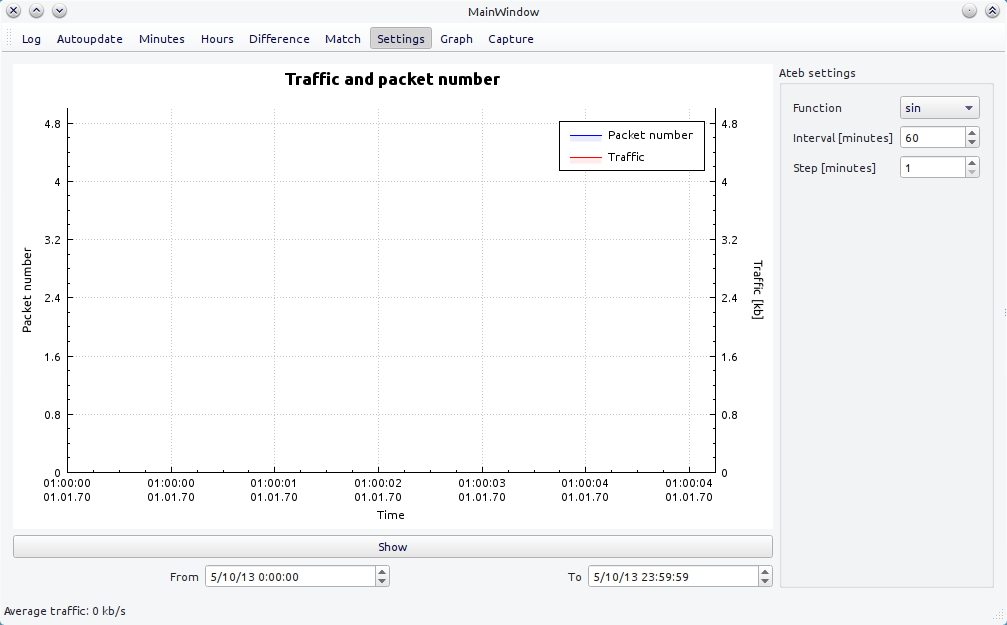
\includegraphics[height=0.4\textheight, width=0.9\textwidth]{fig1}
\caption{The interface of developed software system}
\label{fig:1}
\end{figure}

As shown in Figure~\ref{fig:1} the menu provides the following options:Show – to show traffic data across time marks To and From; Log - logarithmic scale of Scale Y; Autoupdate – to show data for the last 10 minutes with automatic updates; Minutes – to show data on the scale of minutes; Hours – to show data on the scale of hours; Difference – to show the difference between a given Ateb-function and traffic; Match – to show graphs of traffic and Ateb-function simultaneously; Graph – to open an interface to work with graphs; Capture – to open an interface to capture traffic; Settings - see sidebar; Ateb settings - s Ateb function ettings, its type, range and step for computing in Difference mode.
In addition, developed software makes it possible to predict the traffic flow parameters for more efficient use of nodal equipment in the segment computer network.
Now describe the algorithm of work of the software. Initially the observation time T for the flow of traffic and time $t_0$-tick-interval are set. Observation time T is limited by the capabilities of the hardware and can be chosen arbitrarily. Time $t_0$-tick-interval is set within the range specified in the data capture and may be in the range of 0,001s to 10 minutes. The developed software allows analyze and store data traffic. There is a search for the minimum and maximum values of traffic in corresponding moment of time during a given tick-interval. The next step is to find the average value (on the axis OY, along the axis OX preset interval is displayed on the interval $[-\Pi (n, 1), \Pi (n, 1)]$, where $\Pi (n, 1)$ – Ateb-function period) between the minimum and the maximum, to make a comparison with a selected in program Ateb-function. The average value should be zero, and the maximum and minimum respectively 1 and -1, as a limit of Ateb-functions value. All intermediate values are normalized by dividing by half of the difference between the maximum and minimum values of traffic.
Lets introduce into consideration arrays $P = \{P_i | i = 1, \ldots, 100\}$ and $Q = \{Q_i | i = 1, \ldots, 100\}$ that are containing values of traffic flow and calculated values of selected Ateb-function during tick-interval $t_0$. The next step is calculating the difference $| P_i-Q_i |$ between the stored values $P_i$ and the calculated values of the selected Ateb-function $Q_i$ at the selected interval with step $t_0 / 100$, i.e. the number of points of calculation J = 100. Then it searches the mean deviation in the array created differences. The mean deviation is calculated as following:

\begin{equation}
\mu = \frac{\sum_{i=1}^{J}|P_i - Q_i|}{J}
\end{equation}

Then by the equation:
\begin{equation}
M = \frac{2-\mu}{2}
\end{equation}

is recalculated of ordinate value of point for plotting the graph of similarity of Ateb-function  to real traffic flow values during the observation time T. Block diagram of the algorithm of work of developed software system is shown in Figure~\ref{fig:2}.

\begin{figure}
\centering
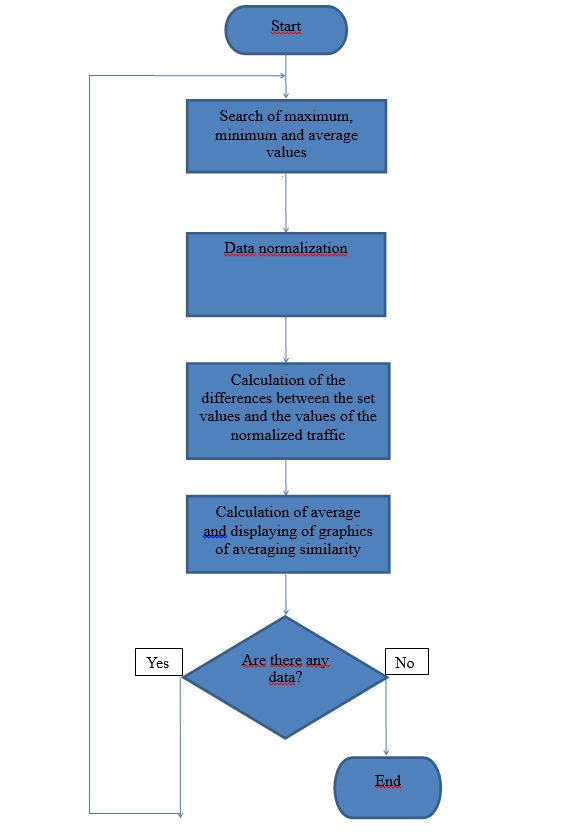
\includegraphics[height=0.9\textheight, width=0.9\textwidth]{fig2}
\caption{Flow chart of developed program working mechanism, responsible for forecasting of traffic flow in the segment of computer network.}
\label{fig:2}
\end{figure}

\section{The Application and Experiments}

The method of analysis and forecasting of traffic flow in the segment of computer network is based on differential equations of oscillating motion. To achieve the this goal, which was in creating a software package for analysis and forecasting of traffic flow in the segment of computer network, which through new actions could reduce packet loss in the hub equipment.

\begin{table}
\caption{Description of customizable features to perform forecasting of traffic flow in the segment of computer network}
{%
\newcommand{\mc}[3]{\multicolumn{#1}{#2}{#3}}
\begin{center}
\small
\begin{tabularx}{\linewidth}[]{|p{0.155\linewidth}|p{0.15\linewidth}|p{0.2\linewidth}|p{0.25\linewidth}|p{0.2\linewidth}|}
\hline
\# & Function & Interval (min) & Step of prediction (min) & Observation time\\
\hline
1 & Sa(1/3, 1) & 60 & 1 & 300 \\
\hline
2 & Sa(1/5, 1) & 60 & 1 & 300 \\
\hline
3 & Sa(1/7, 3) & 60 & 1 & 300 \\
\hline
4 & Sin & 60 & 1 & 300 \\
\hline
\end{tabularx}
\end{center}
}%
\end{table}


%\begin{figure}
%\centering
%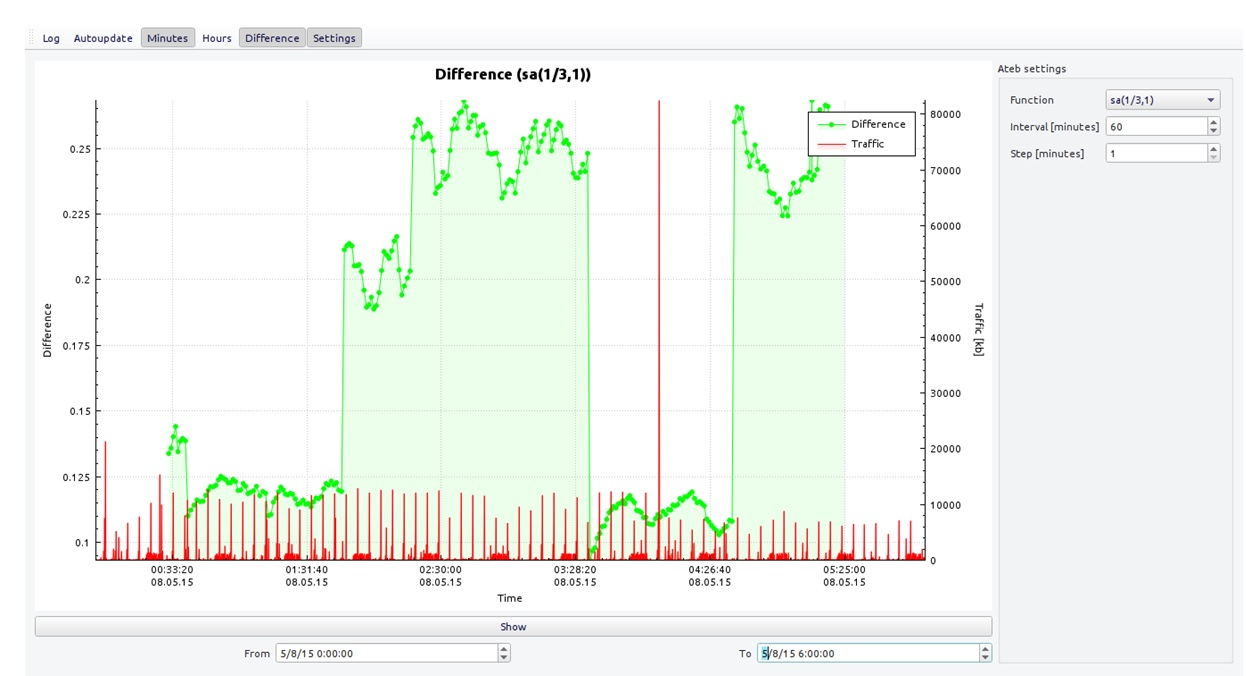
\includegraphics[height=0.1\textheight, width=0.1\textwidth]{fig3}
%\caption{}
%\label{fig:3}
%\end{figure}

%\begin{figure}
%\centering
%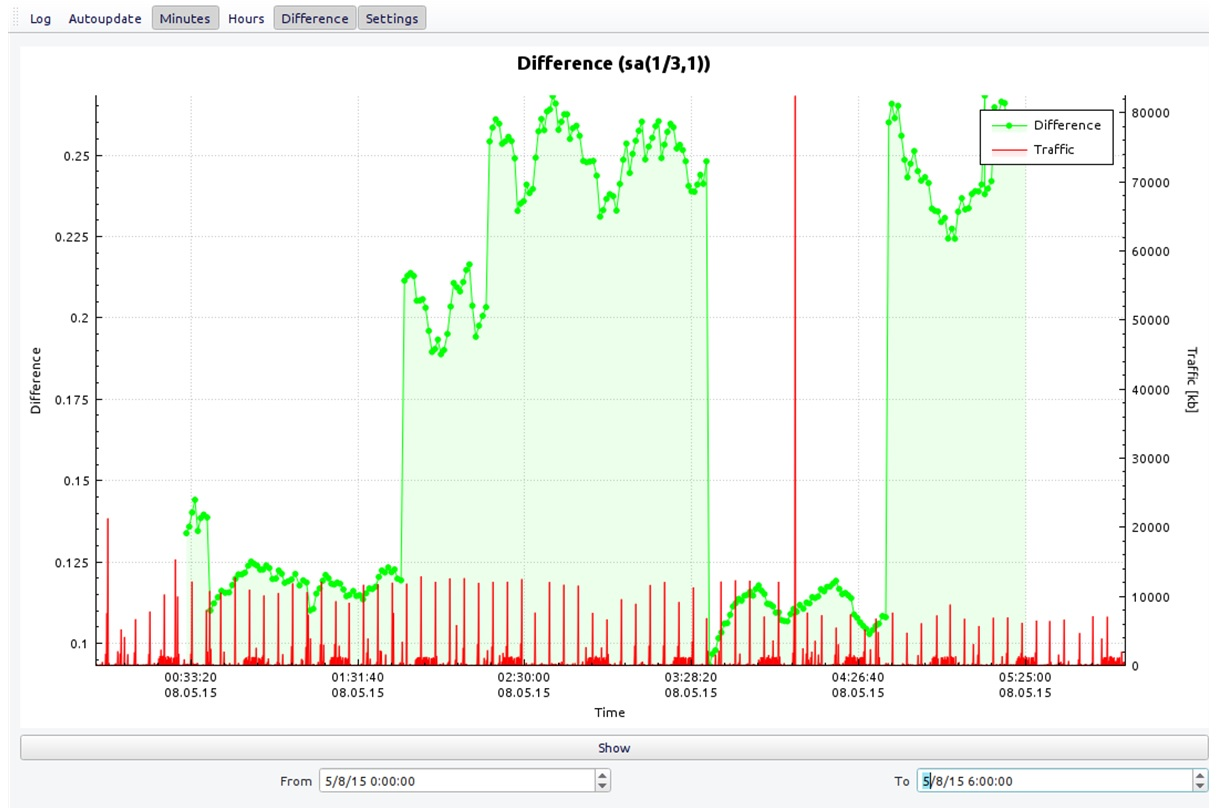
\includegraphics[height=0.1\textheight, width=0.1\textwidth]{fig4}
%\caption{}
%\label{fig:4}
%\end{figure}

%\begin{figure}
%\centering
%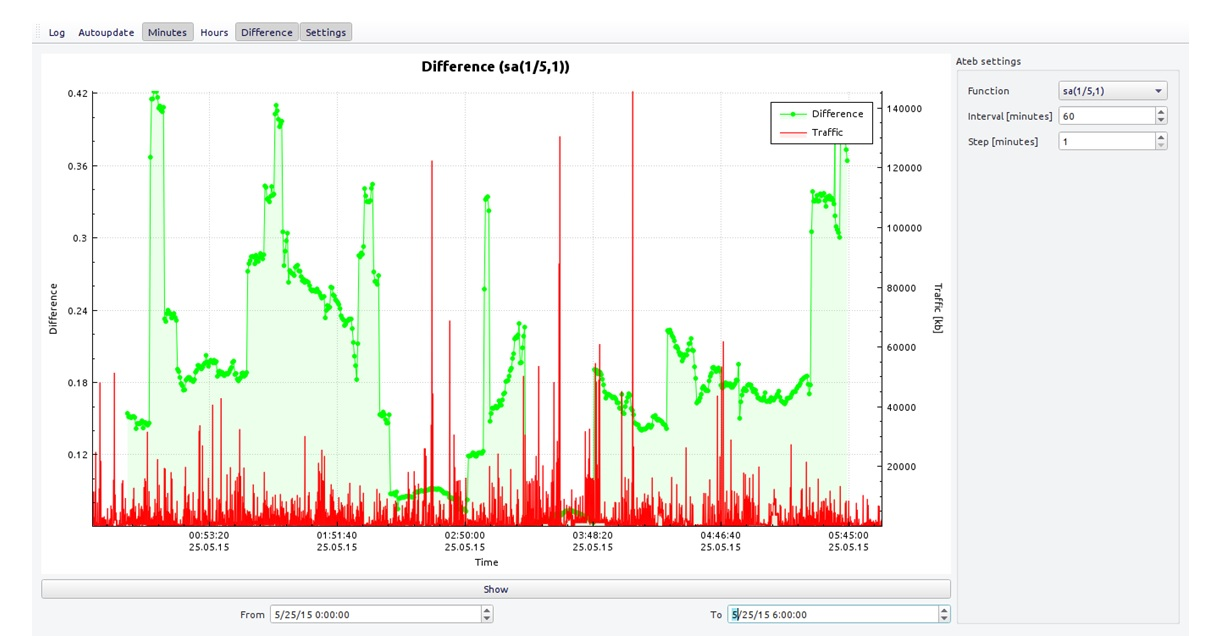
\includegraphics[height=0.1\textheight, width=0.1\textwidth]{fig5}
%\caption{}
%\label{fig:5}
%\end{figure}

%\begin{figure}
%\centering
%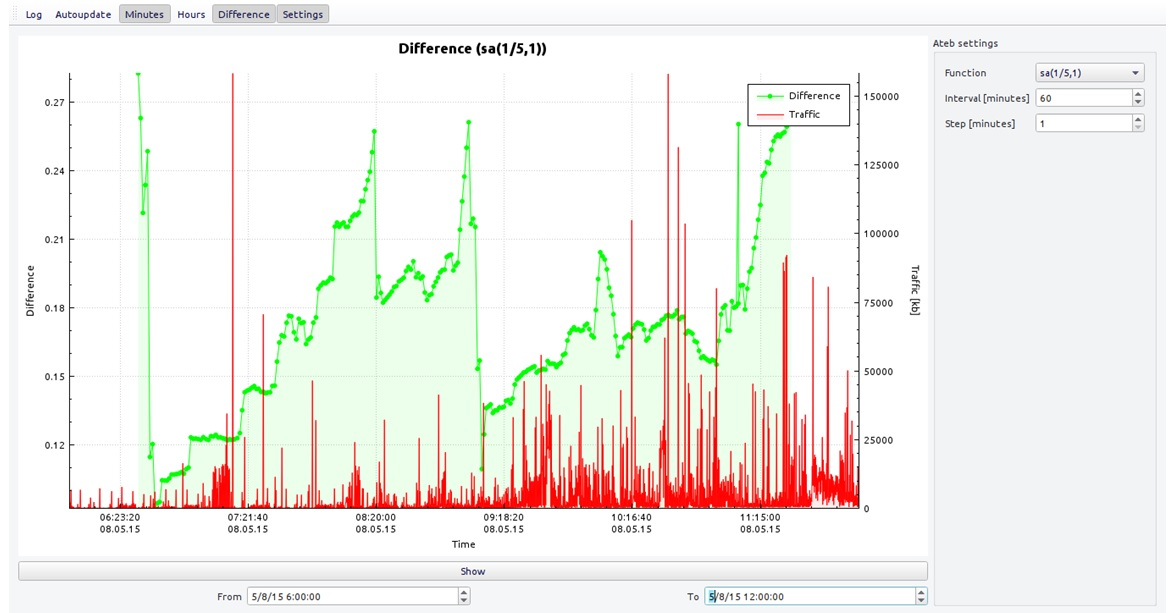
\includegraphics[height=0.1\textheight, width=0.1\textwidth]{fig6}
%\caption{}
%\label{fig:6}
%\end{figure}

\section{Network Topology}
On the next figure the topology of computer network of ACS Department in Lviv Polytechnic National University is presented. Switches that are used in network of ACS department are the following:
\begin{enumerate}
  \item D-Link DES – 1024 R
  \item 3Com Swich 3300 xM
  \item 3Com Swich 4226 T
  \item Allied Telesyn AT8026T
\end{enumerate}

%\begin{figure}
%\centering
%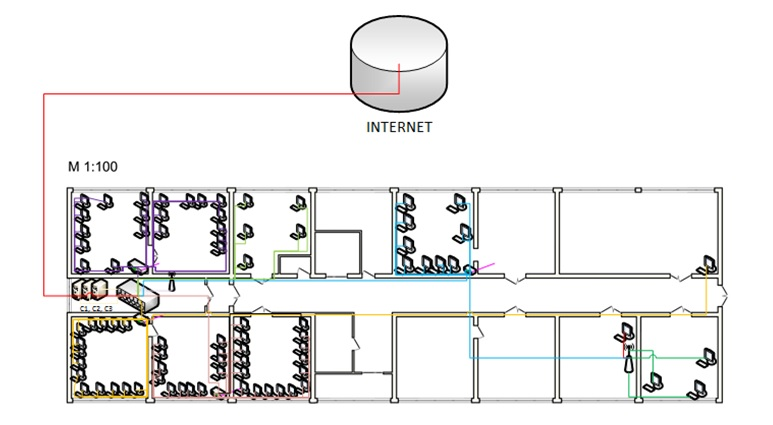
\includegraphics[height=0.1\textheight, width=0.1\textwidth]{fig7}
%\caption{The topology of computer network of ACS Department}
%\label{fig:7}
%\end{figure}

\section{The Research Results}

To calculate the results of the experiment, the following equations which are describing the maximum correlation and coefficient that shows the ratio of standard deviation to the maximum were chosen.
Equations that were used for computing:
The maximum correlation ρ:

\begin{equation}
r_{xy} = \frac{ \sum_{i=1}^{m} (x_i - \overline{x})(y_i - \overline{y}) }{ \sqrt{(x_i - \overline{x}) ^ 2 \sum_{i=1}^{m} (y_i - \overline{y})^2 }} = \frac{cov(x,y)}{\sqrt{s_x^2 s_y^2}}
\end{equation}

where $\rho = \max_{x} r_{xy}$,  $r_{xy} \in A$

Coefficient  К of ratio of standard deviation to maximum:
\begin{equation}
K = \frac{s_{max}}{s}
\end{equation}

where
\begin{equation}
s = \sqrt{ \frac{n}{n-1} \sigma ^2 } = \sqrt{ \frac{1}{n-1} \sum_{i=1}^n (x_i - \overline{x})^2}
\end{equation}

Comparison of simulation experiments E1, E2, E3 conducted by the criterion of maximum correlation ρ, and also was calculated coefficient k of ratio of standard deviation to the maximum. The calculated results of the comparison are presented in Table 2.

\begin{table}
\caption{Comparison of traffic simulation results with real data network traffic of ACS department in Lviv Polytechnic for 1 day}
{%
\newcommand{\mc}[3]{\multicolumn{#1}{#2}{#3}}
\begin{center}
\small
\begin{tabularx}{\linewidth}[]{|p{0.24\linewidth}|p{0.24\linewidth}|p{0.24\linewidth}|p{0.24\linewidth}|}
\hline
\ Variable & E1 & E2 & E3\\
\hline
  K & 10.81 & 12.56 & 12.75\\
\hline
  $\rho$ & 0.79 & 0.75 & 0.74\\
\hline
\end{tabularx}
\end{center}
}%
\end{table}

The maximum amplitude of perturbation function was changed - experiment E2 and the number of disturbances - experiment E3. Apparently, the best results were obtained for model experiment data in experiment E1. (Is that sentence needed?)

\section{Conclusion}
This article describes developed by authors the software system for the simulation of traffic flow for TCP / IP networks based on mathematical model, which is based on differential equations of oscillating motion with one degree of freeness. Interface of the software system, and the algorithm of its work were presented and described. Testing of software system was implemented in the computer network  of NULP ACS department. Topology of TCP / IP network in this department was presented. The results of the program while working were graphically illustrated. The relationship between real and simulated traffic was shown. Parameters of correlation between the real and calculated by formulas traffic were calculated. 
%Presented calculations show that the real and calculated traffic is different for.......... 
%Conducted also experimental calculations in depending on the averaging of real time, are showing .............
%Received results will be used to create the unit for optimal control of switch with the aim of improving the use of nodular equipment.

\section{References}

\begin{thebibliography}{6}

\bibitem{1} Cisco Visual Networking Index Predicts IP Traffic to Triple from 2014-2019, \url{http://newsroom.cisco.com}

\bibitem{2} E. Morozov, R.Nekrasova, L.Potakhina, O. Tikhonenko Asymptotic Analysis of Queueing Systems with Finite Buffer Space // CN 2014, CCIS 431, pp. 223-232

\bibitem{3} J.Domanska, A.Domanski, T. Czachorski Modelling Packet Traffic with the Use of Superpositions of Two-State MMPPs// CN 2014, CCIS 431, pp. 24-36.

\bibitem{4} T.Czachórski, F. Pekergin Diffusion Approximation as a Modelling Tool // Network Performance EngineeringVol. 5233 of the series Lecture Notes in Computer Science, pp 447-476.

\bibitem{5} I. M. Droniuk, M. A. Nazarkevich Мodeling nonlinear oscillatory system under disturbance by means of Ateb-functions for the Internet  // Proceedings of 6th working international conference «Het-Nets 2010». — Gliwice, 2009. — p. 325–335.

\bibitem{6} Ivanna Dronjuk, Maria Nazarkevych, Olga Fedevych. Asymptotic method of traffic simulation (Distributed Computer and Communication Networks) // Communications in Computer and Information Science. Springer 2014, Vol. 279, pp.136-144.

\end{thebibliography}



\subsection{Program Code}

Program listings or program commands in the text are normally set in
typewriter font, e.g., CMTT10 or Courier.

\medskip

\noindent
{\it Example of a Computer Program}
\begin{verbatim}
program Inflation (Output)
  {Assuming annual inflation rates of 7%, 8%, and 10%,...
   years};
   const
     MaxYears = 10;
   var
     Year: 0..MaxYears;
     Factor1, Factor2, Factor3: Real;
   begin
     Year := 0;
     Factor1 := 1.0; Factor2 := 1.0; Factor3 := 1.0;
     WriteLn('Year  7% 8% 10%'); WriteLn;
     repeat
       Year := Year + 1;
       Factor1 := Factor1 * 1.07;
       Factor2 := Factor2 * 1.08;
       Factor3 := Factor3 * 1.10;
       WriteLn(Year:5,Factor1:7:3,Factor2:7:3,Factor3:7:3)
     until Year = MaxYears
end.
\end{verbatim}
%
\noindent
{\small (Example from Jensen K., Wirth N. (1991) Pascal user manual and
report. Springer, New York)}

\subsection{Citations}

For citations in the text please use
square brackets and consecutive numbers: \cite{jour}, \cite{lncschap},
\cite{proceeding1} -- provided automatically
by \LaTeX 's \verb|\cite| \dots\verb|\bibitem| mechanism.


%%% Local Variables:
%%% mode: latex
%%% TeX-master: t
%%% End:
\end{document}